% Options for packages loaded elsewhere
\PassOptionsToPackage{unicode}{hyperref}
\PassOptionsToPackage{hyphens}{url}
\PassOptionsToPackage{dvipsnames,svgnames,x11names}{xcolor}
%
\documentclass[
  12pt,
]{article}
\usepackage{amsmath,amssymb}
\usepackage{lmodern}
\usepackage{iftex}
\ifPDFTeX
  \usepackage[T1]{fontenc}
  \usepackage[utf8]{inputenc}
  \usepackage{textcomp} % provide euro and other symbols
\else % if luatex or xetex
  \usepackage{unicode-math}
  \defaultfontfeatures{Scale=MatchLowercase}
  \defaultfontfeatures[\rmfamily]{Ligatures=TeX,Scale=1}
\fi
% Use upquote if available, for straight quotes in verbatim environments
\IfFileExists{upquote.sty}{\usepackage{upquote}}{}
\IfFileExists{microtype.sty}{% use microtype if available
  \usepackage[]{microtype}
  \UseMicrotypeSet[protrusion]{basicmath} % disable protrusion for tt fonts
}{}
\makeatletter
\@ifundefined{KOMAClassName}{% if non-KOMA class
  \IfFileExists{parskip.sty}{%
    \usepackage{parskip}
  }{% else
    \setlength{\parindent}{0pt}
    \setlength{\parskip}{6pt plus 2pt minus 1pt}}
}{% if KOMA class
  \KOMAoptions{parskip=half}}
\makeatother
\usepackage{xcolor}
\usepackage[margin=1in]{geometry}
\usepackage{longtable,booktabs,array}
\usepackage{calc} % for calculating minipage widths
% Correct order of tables after \paragraph or \subparagraph
\usepackage{etoolbox}
\makeatletter
\patchcmd\longtable{\par}{\if@noskipsec\mbox{}\fi\par}{}{}
\makeatother
% Allow footnotes in longtable head/foot
\IfFileExists{footnotehyper.sty}{\usepackage{footnotehyper}}{\usepackage{footnote}}
\makesavenoteenv{longtable}
\usepackage{graphicx}
\makeatletter
\def\maxwidth{\ifdim\Gin@nat@width>\linewidth\linewidth\else\Gin@nat@width\fi}
\def\maxheight{\ifdim\Gin@nat@height>\textheight\textheight\else\Gin@nat@height\fi}
\makeatother
% Scale images if necessary, so that they will not overflow the page
% margins by default, and it is still possible to overwrite the defaults
% using explicit options in \includegraphics[width, height, ...]{}
\setkeys{Gin}{width=\maxwidth,height=\maxheight,keepaspectratio}
% Set default figure placement to htbp
\makeatletter
\def\fps@figure{htbp}
\makeatother
\setlength{\emergencystretch}{3em} % prevent overfull lines
\providecommand{\tightlist}{%
  \setlength{\itemsep}{0pt}\setlength{\parskip}{0pt}}
\setcounter{secnumdepth}{-\maxdimen} % remove section numbering
\usepackage[english]{babel}
\usepackage[utf8]{inputenc}
\usepackage{csquotes}
\usepackage{fancyhdr}
\usepackage{setspace}
\usepackage{geometry}
\usepackage{verbatim}
\usepackage{hyperref}
\usepackage{xcolor}
\usepackage{floatrow}
\floatsetup[table]{capposition=top}
\floatsetup[figure]{capposition=top}
\usepackage{booktabs}
\usepackage{longtable}
\usepackage{array}
\usepackage{multirow}
\usepackage{wrapfig}
\usepackage{float}
\usepackage{colortbl}
\usepackage{pdflscape}
\usepackage{tabu}
\usepackage{threeparttable}
\usepackage{threeparttablex}
\usepackage[normalem]{ulem}
\usepackage{makecell}
\usepackage{xcolor}
\ifLuaTeX
  \usepackage{selnolig}  % disable illegal ligatures
\fi
\usepackage[backend=biber,citestyle=authoryear,maxcitenames=2,useprefix,autocite=inline,doi=false,url=false,isbn=false]{biblatex}
\addbibresource{../bibliography/nottingham-rep.bib}
\IfFileExists{bookmark.sty}{\usepackage{bookmark}}{\usepackage{hyperref}}
\IfFileExists{xurl.sty}{\usepackage{xurl}}{} % add URL line breaks if available
\urlstyle{same} % disable monospaced font for URLs
\hypersetup{
  pdftitle={Replication of @Frederiksen2022a},
  pdfauthor={Tom Brailey},
  colorlinks=true,
  linkcolor={blue},
  filecolor={Maroon},
  citecolor={Blue},
  urlcolor={Blue},
  pdfcreator={LaTeX via pandoc}}

\title{Replication of \textcite{Frederiksen2022a}}
\author{Tom Brailey\footnote{Word count: 136}}
\date{March, 2023}

\begin{document}
\maketitle

{
\hypersetup{linkcolor=}
\setcounter{tocdepth}{2}
\tableofcontents
}
\hypertarget{introduction}{%
\section{Introduction}\label{introduction}}

This memo begins by replicating the main exhibits in \textcite{Frederiksen2022a} (as well as some of the exhibits in their supplementary materials section\footnote{See \autocite{Frederiksen2022b,Frederiksen2022c}}) using the R programming language.

\hypertarget{replication}{%
\section{Replication}\label{replication}}

\hypertarget{replication-of-main-exhibits}{%
\subsection{Replication of Main Exhibits}\label{replication-of-main-exhibits}}

The main paper only contains one exhibit, Figure 1, replicated below. The figure replicates exactly, though it should be noted that the the upper panels of Figure 1 are calculated without reference to a base category, while the lower panels are the marginal means compared to the third category of the independent variable (\texttt{cancom}).

\begin{figure}
\centering
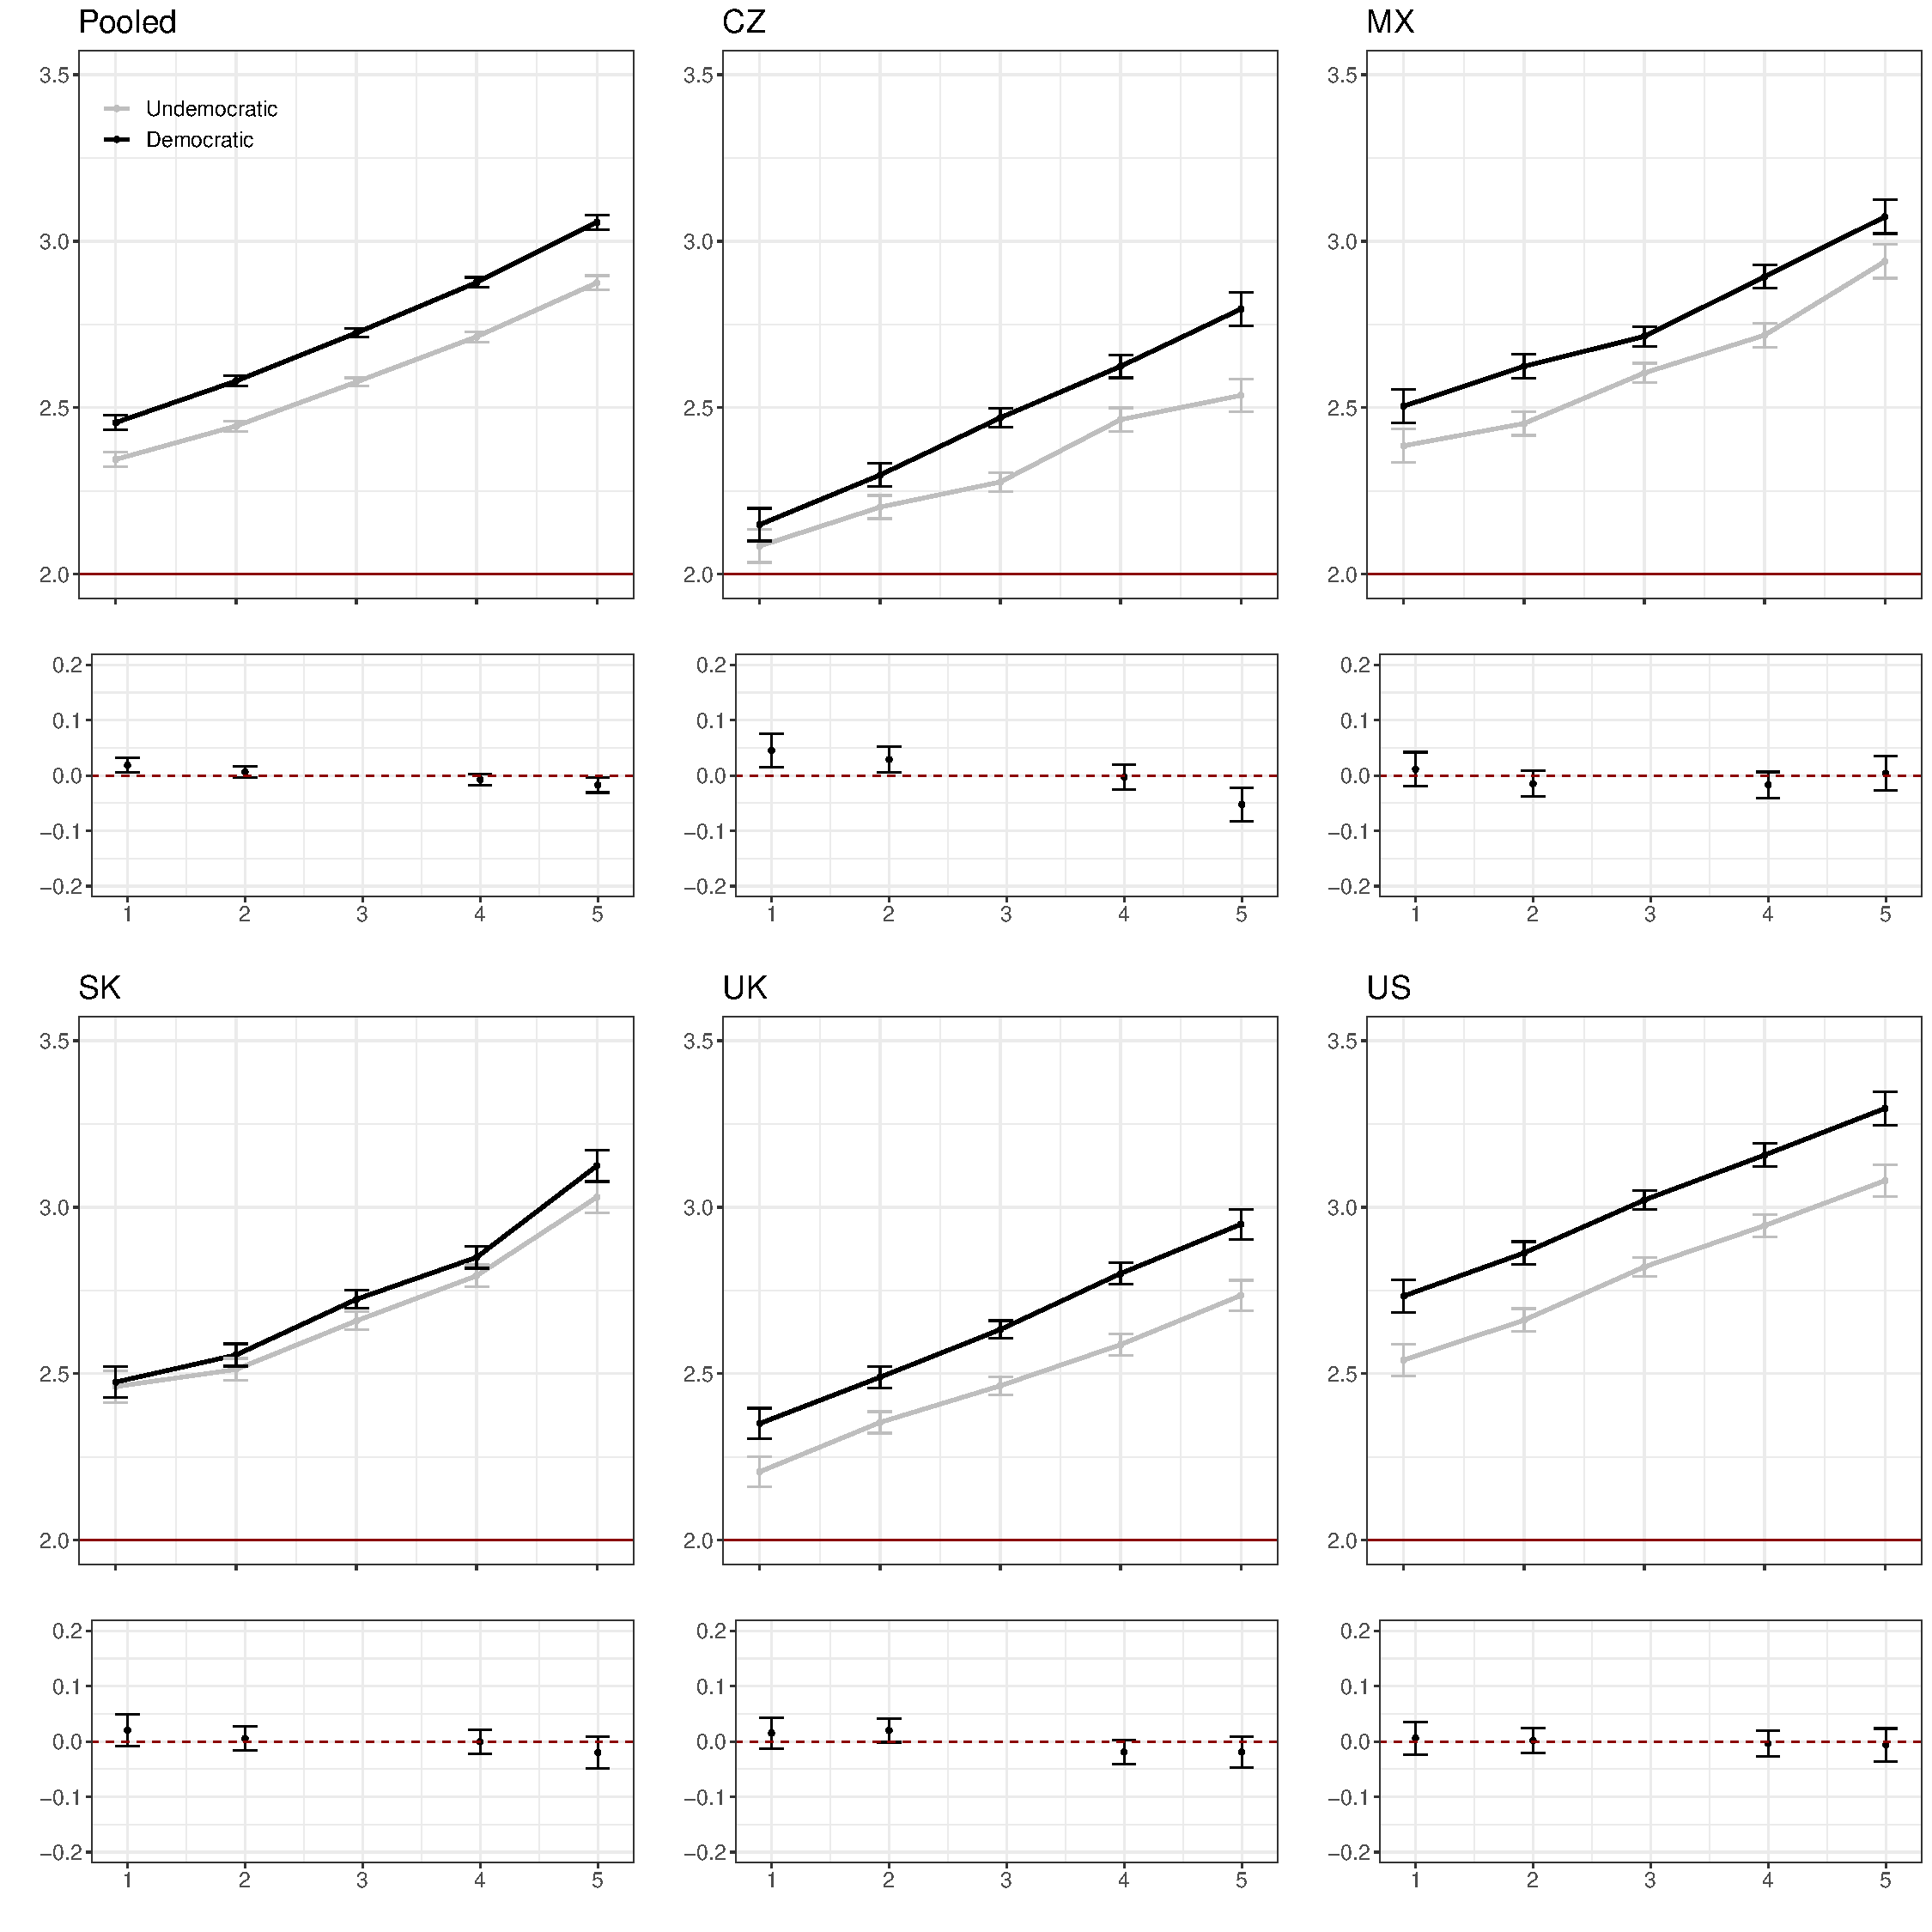
\includegraphics{../exhibits/figures/figure1_replication.pdf}
\caption{\label{fig:unnamed-chunk-2}Replication of Figure 1}
\end{figure}

\clearpage

\hypertarget{replication-of-dataverse-appendix-a}{%
\subsection{Replication of Dataverse Appendix A}\label{replication-of-dataverse-appendix-a}}

Both tables in Appendix A replicate exactly in terms of point estimates, statistical significance, and number of observations.


\begin{table}[!htbp]
\caption{Average effects of undemocratic behavior andcompetence in the Czech Republic, Mexico, South Korea, the UnitedKingdom, and the United States. Candidate support is the dependentvariable in all models.}
\begin{center}
\begin{tabular}{l c c c c c}
\hline
 & Model 1 & Model 2 & Model 3 & Model 4 & Model 5 \\
\hline
Undemocratic behavior & $-0.15^{***}$ & $-0.16^{***}$ & $-0.14^{***}$ & $-0.06^{***}$ & $-0.17^{***}$ \\
                      & $(0.01)$      & $(0.01)$      & $(0.01)$      & $(0.01)$      & $(0.01)$      \\
Very incompetent      & $-0.25^{***}$ & $-0.26^{***}$ & $-0.21^{***}$ & $-0.22^{***}$ & $-0.27^{***}$ \\
                      & $(0.01)$      & $(0.02)$      & $(0.02)$      & $(0.02)$      & $(0.02)$      \\
Incompetent           & $-0.14^{***}$ & $-0.12^{***}$ & $-0.12^{***}$ & $-0.16^{***}$ & $-0.13^{***}$ \\
                      & $(0.01)$      & $(0.02)$      & $(0.02)$      & $(0.02)$      & $(0.02)$      \\
Competent             & $0.14^{***}$  & $0.17^{***}$  & $0.15^{***}$  & $0.13^{***}$  & $0.15^{***}$  \\
                      & $(0.01)$      & $(0.02)$      & $(0.02)$      & $(0.02)$      & $(0.02)$      \\
Very Competent        & $0.31^{***}$  & $0.29^{***}$  & $0.35^{***}$  & $0.39^{***}$  & $0.29^{***}$  \\
                      & $(0.01)$      & $(0.02)$      & $(0.02)$      & $(0.02)$      & $(0.02)$      \\
Constant              & $2.72^{***}$  & $2.45^{***}$  & $2.73^{***}$  & $2.72^{***}$  & $2.64^{***}$  \\
                      & $(0.01)$      & $(0.02)$      & $(0.02)$      & $(0.02)$      & $(0.02)$      \\
\hline
R$^2$                 & $0.02$        & $0.02$        & $0.02$        & $0.02$        & $0.02$        \\
Adj. R$^2$            & $0.02$        & $0.02$        & $0.02$        & $0.02$        & $0.02$        \\
Num. obs.             & $267795$      & $47221$       & $55167$       & $50002$       & $55299$       \\
RMSE                  & $1.36$        & $1.29$        & $1.43$        & $1.26$        & $1.29$        \\
N Clusters            & $14058$       & $2481$        & $2845$        & $2691$        & $2882$        \\
\hline
\multicolumn{6}{l}{\scriptsize{$^{***}p<0.001$; $^{**}p<0.01$; $^{*}p<0.05$}}
\end{tabular}
\label{table_a1}
\end{center}
\end{table}



\begin{table}[!htbp]
\caption{Table A1}
\begin{center}
\begin{tabular}{l c c c c c}
\hline
 & Model 1 & Model 2 & Model 3 & Model 4 & Model 5 \\
\hline
Undemocratic behavior           & $-0.15^{***}$ & $-0.19^{***}$ & $-0.11^{***}$ & $-0.06^{***}$ & $-0.17^{***}$ \\
                                & $(0.01)$      & $(0.02)$      & $(0.02)$      & $(0.02)$      & $(0.02)$      \\
Very incompetent                & $-0.27^{***}$ & $-0.32^{***}$ & $-0.21^{***}$ & $-0.25^{***}$ & $-0.28^{***}$ \\
                                & $(0.01)$      & $(0.03)$      & $(0.03)$      & $(0.03)$      & $(0.03)$      \\
Incompetent                     & $-0.14^{***}$ & $-0.17^{***}$ & $-0.09^{***}$ & $-0.17^{***}$ & $-0.14^{***}$ \\
                                & $(0.01)$      & $(0.02)$      & $(0.02)$      & $(0.02)$      & $(0.02)$      \\
Very competent                  & $0.15^{***}$  & $0.15^{***}$  & $0.18^{***}$  & $0.13^{***}$  & $0.17^{***}$  \\
                                & $(0.01)$      & $(0.02)$      & $(0.02)$      & $(0.02)$      & $(0.02)$      \\
Undemocratic x Very incompetent & $0.04^{*}$    & $0.13^{**}$   & $-0.01$       & $0.05$        & $0.02$        \\
                                & $(0.02)$      & $(0.04)$      & $(0.04)$      & $(0.04)$      & $(0.04)$      \\
Undemocratic x Incompetent      & $0.01$        & $0.10^{**}$   & $-0.06$       & $0.02$        & $0.03$        \\
                                & $(0.01)$      & $(0.03)$      & $(0.03)$      & $(0.03)$      & $(0.03)$      \\
Undemocratic x Competent        & $-0.02$       & $0.03$        & $-0.07^{*}$   & $0.01$        & $-0.04$       \\
                                & $(0.01)$      & $(0.03)$      & $(0.03)$      & $(0.03)$      & $(0.03)$      \\
Undemocratic x Very competent   & $-0.03$       & $-0.07$       & $-0.02$       & $-0.03$       & $-0.04$       \\
                                & $(0.02)$      & $(0.04)$      & $(0.04)$      & $(0.04)$      & $(0.04)$      \\
\hline
R$^2$                           & $0.02$        & $0.02$        & $0.02$        & $0.02$        & $0.02$        \\
Adj. R$^2$                      & $0.02$        & $0.02$        & $0.02$        & $0.02$        & $0.02$        \\
Num. obs.                       & $267795$      & $47221$       & $55167$       & $50002$       & $55299$       \\
RMSE                            & $1.36$        & $1.29$        & $1.43$        & $1.26$        & $1.29$        \\
N Clusters                      & $14058$       & $2481$        & $2845$        & $2691$        & $2882$        \\
\hline
\multicolumn{6}{l}{\scriptsize{$^{***}p<0.001$; $^{**}p<0.01$; $^{*}p<0.05$}}
\end{tabular}
\label{table:coefficients}
\end{center}
\end{table}


\clearpage

\hypertarget{replication-of-supplementary-materials-appendix-a}{%
\subsection{Replication of Supplementary Materials Appendix A}\label{replication-of-supplementary-materials-appendix-a}}

\begin{longtable}[t]{>{\raggedright\arraybackslash}p{7cm}rrrrr}
\caption{\label{tab:unnamed-chunk-3}Distribution of attributes: US, UK, and CZ. Age is drawn randomly from probability-specified intervals.}\\
\toprule
Attribute Category & CZ & UK & US & MX & SK\\
\midrule
\endfirsthead
\caption[]{\label{tab:unnamed-chunk-3}Distribution of attributes: US, UK, and CZ. Age is drawn randomly from probability-specified intervals. \textit{(continued)}}\\
\toprule
Attribute Category & CZ & UK & US & MX & SK\\
\midrule
\endhead

\endfoot
\bottomrule
\endlastfoot
43-57 & 0.333 & NA & NA & NA & NA\\
58-67 & 0.334 & NA & NA & NA & NA\\
68-77 & 0.334 & NA & NA & NA & NA\\
44-53 & NA & 0.332 & NA & NA & NA\\
54-57 & NA & 0.336 & NA & NA & NA\\
\addlinespace
58-61 & NA & 0.332 & NA & NA & NA\\
40-49 & NA & NA & 0.198 & NA & NA\\
50-59 & NA & NA & 0.200 & NA & NA\\
60-62 & NA & NA & 0.199 & NA & NA\\
63-66 & NA & NA & 0.201 & NA & NA\\
\addlinespace
67-75 & NA & NA & 0.201 & NA & NA\\
Female & 0.083 & 0.286 & 0.202 & 0.126 & 0.055\\
Male & 0.917 & 0.714 & 0.798 & 0.874 & 0.945\\
Actor/actress & 0.169 & NA & NA & NA & NA\\
Journalist & 0.252 & 0.224 & NA & 0.032 & 0.055\\
\addlinespace
Political Career & 0.084 & 0.222 & 0.101 & NA & 0.112\\
Professor & 0.496 & NA & NA & NA & 0.055\\
Academic & NA & NA & NA & 0.031 & NA\\
Accountant & NA & NA & NA & 0.124 & NA\\
Business Administration & NA & NA & NA & 0.061 & NA\\
\addlinespace
Civil Servant & NA & 0.111 & 0.101 & 0.094 & 0.056\\
Engineer & NA & NA & NA & 0.127 & 0.056\\
Lawyer & NA & 0.221 & 0.301 & 0.407 & 0.387\\
Professional Sports & NA & NA & NA & 0.031 & NA\\
Self-employed & NA & NA & 0.098 & 0.093 & 0.167\\
\addlinespace
Army General & NA & NA & NA & NA & 0.056\\
Company Director & NA & NA & NA & NA & 0.055\\
Banker & NA & 0.222 & NA & NA & NA\\
Company Founder/Director & NA & NA & 0.399 & NA & NA\\
ANO 2011 & 0.336 & NA & NA & NA & NA\\
\addlinespace
ODS (Občanská demokratická strana) & 0.333 & NA & NA & NA & NA\\
ČSSD (Česká strana sociálně demokratická) & 0.331 & NA & NA & NA & NA\\
MORENA & NA & NA & NA & 0.249 & NA\\
PAN & NA & NA & NA & 0.249 & NA\\
PRD & NA & NA & NA & 0.251 & NA\\
\addlinespace
PRI & NA & NA & NA & 0.251 & NA\\
Democratic Party of Korea & NA & NA & NA & NA & 0.499\\
United Future Party & NA & NA & NA & NA & 0.501\\
Conservatives & NA & 0.502 & NA & NA & NA\\
Labour & NA & 0.498 & NA & NA & NA\\
\addlinespace
Democrat & NA & NA & 0.501 & NA & NA\\
Republican & NA & NA & 0.499 & NA & NA\\
Decrease income tax on 10 percent richest & 0.167 & 0.163 & 0.166 & 0.166 & 0.169\\
Decrease power of labor unions & 0.169 & NA & 0.169 & NA & 0.167\\
Decrease public welfare spending & 0.164 & 0.165 & 0.166 & 0.165 & 0.167\\
\addlinespace
Increase income tax on 10 percent richest & 0.163 & 0.168 & 0.165 & 0.169 & 0.167\\
Increase power of labor unions & 0.168 & NA & 0.165 & NA & 0.165\\
Increase public welfare spending & 0.169 & 0.169 & 0.168 & 0.158 & 0.166\\
Prevent universal access to public colleges & NA & NA & NA & 0.166 & NA\\
Provide universal access to public colleges & NA & NA & NA & 0.177 & NA\\
\addlinespace
Decrease power of trade unions & NA & 0.168 & NA & NA & NA\\
Increase power of trade unions & NA & 0.166 & NA & NA & NA\\
Allow illegal immigrants to apply for citizenship & 0.166 & 0.167 & 0.168 & NA & NA\\
Increase efforts to arrest and eventually deport illegal immigrants & 0.167 & 0.165 & 0.164 & NA & NA\\
Make it easier for people of the same sex to marry each other & 0.166 & 0.168 & 0.164 & NA & NA\\
\addlinespace
Make it easier for women to get an abortion & 0.166 & 0.166 & 0.168 & NA & NA\\
Make it harder for people of the same sex to marry each other & 0.168 & 0.166 & 0.168 & NA & NA\\
Make it harder for women to get an abortion & 0.168 & 0.168 & 0.168 & NA & NA\\
Legalize same-sex marriage nationally & NA & NA & NA & 0.169 & 0.167\\
Make abortion law more strict & NA & NA & NA & 0.166 & 0.167\\
\addlinespace
Prohibit same-sex marriage nationally & NA & NA & NA & 0.167 & 0.168\\
Provide amnesty to low-level drug offenders & NA & NA & NA & 0.166 & NA\\
Punish all drug-related crime harsher & NA & NA & NA & 0.165 & NA\\
Relax abortion law & NA & NA & NA & 0.166 & 0.168\\
Decrease funds to the army & NA & NA & NA & NA & 0.166\\
\addlinespace
Increase funds to the army & NA & NA & NA & NA & 0.165\\
Said court rulings by judges appointed by opposing parties should be adhered to & 0.125 & 0.127 & 0.124 & 0.125 & 0.126\\
Said court rulings by judges appointed by opposing parties should be ignored & 0.125 & 0.124 & 0.125 & 0.125 & 0.123\\
Said it is acceptable to harass journalists that do not reveal sources & 0.125 & 0.123 & 0.124 & 0.124 & 0.124\\
Said it is legitimate to fight political opponents in the streets if one feels provoked & 0.126 & 0.123 & 0.127 & 0.125 & 0.125\\
\addlinespace
Said it is unacceptable to fight political opponents in the streets even though one feels provoked & 0.123 & 0.126 & 0.125 & 0.127 & 0.127\\
Said it is unacceptable to harass journalists even though they do not reveal sources & 0.125 & 0.126 & 0.123 & 0.123 & 0.124\\
Supported a proposal to preserve existing polling-stations in all areas & 0.128 & 0.124 & 0.125 & 0.126 & 0.126\\
Supported a proposal to reduce polling stations in areas that support opposing parties & 0.122 & 0.127 & 0.127 & 0.125 & 0.125\\
Bad at handling economic matters & 0.336 & 0.338 & 0.335 & 0.334 & 0.335\\
\addlinespace
Good at handling economic matters & 0.330 & 0.331 & 0.331 & 0.333 & 0.335\\
Neither good nor bad reputation on economic matters & 0.334 & 0.331 & 0.334 & 0.333 & 0.330\\
Bad at fighting corruption & 0.337 & 0.331 & 0.333 & 0.335 & 0.334\\
Good at fighting corruption & 0.334 & 0.336 & 0.332 & 0.331 & 0.333\\
Neither good nor bad reputation on fighting corruption & 0.329 & 0.333 & 0.335 & 0.335 & 0.333\\*
\end{longtable}

\clearpage

\hypertarget{extension}{%
\section{Extension}\label{extension}}

In this section, I extend the analysis presented in \textcite{Frederiksen2022a}.

\printbibliography

\end{document}
